\chapter{薄板型抗震阻尼器数值模拟分析}
在本章中对工程应用中常见的三种薄板型抗震阻尼器进行介绍,随后通过建模对其进行数值模拟分析,分别使用三种不同的本质边界条件罚函数法、Nitsche法和本文所提的基于赫林格-赖斯纳原理的变分一致性本质边界条件施加方法得到弯矩位移云图进行对比分析,进一步证明所提方法在解决工程应用薄板型抗震阻尼器方面具有的一定优势。
\section{ADAS阻尼器}
在建筑和工程结构中,振动是一个常见的问题,其可能会导致结构的疲劳破坏等问题,传统方法中通过采用增加结构的刚度或使用液体阻尼器、摩擦阻尼器减小结构的振动响应,然而在传统方法中或多或少的存在有效性不高,经济适用性低等问题。
为了克服传统方法的限制,ADAS减振刚度阻尼器被引入,ADAS阻尼器是一种基于能量耗散原理的被动控制装置,通过在结构中引入附加的阻尼力来吸收和耗散结构的振动能量,能够有效地减小结构地的振动幅值和振动周期,从而显著改善结构的振动响应,
并且ADAS阻尼器的设计相对简单,通常由一块或多块金属材料制成,安装简易、价格低廉,是一种在结构工程中广泛应用于减震和控制结构的被动控制装置。\par
图(\ref{ADAS1})、(\ref{ADAS2})分别为ADAS阻尼器与裸框架示意图和ADAS阻尼器的具体尺寸示意图,如图(\ref{ADAS2})所示,ADAS阻尼器中的上端部分设为简支固定,施加本质边界条件$\Gamma^g$,对下端施加$P=100000$,ADAS阻尼器钢板的材料系数分别为杨氏模量$E=2\times 10^{11}$、泊松比$\nu=0.3$。
图()为三种不同本质边界条件施加方法得出的弯矩应力云图,从图中可以看出
\begin{figure}[H]
    \centering
    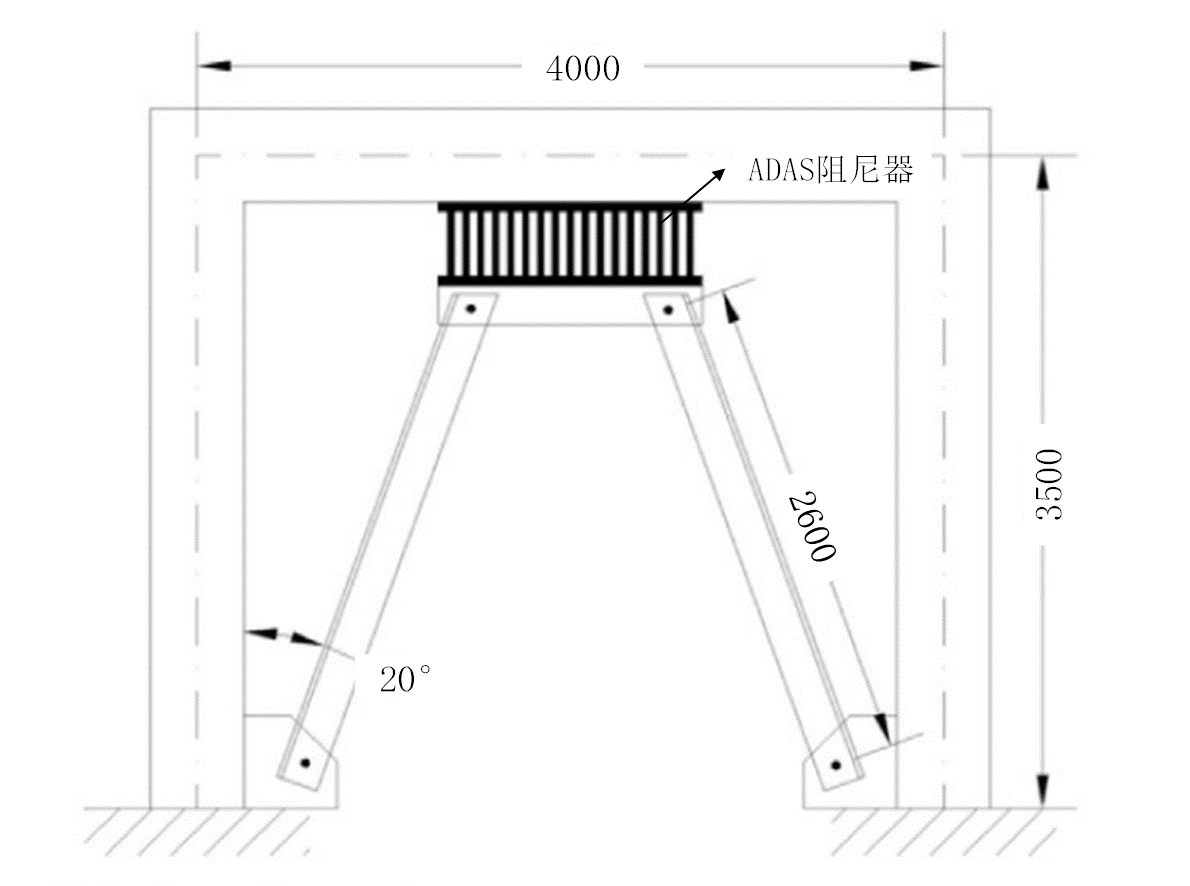
\includegraphics[scale=0.6]{figure/DAMPER/ADAS/1.png}
    \caption{实验装置示意图\cite{basu2016}}\label{ADAS1}
\end{figure}
\begin{figure}[H]
    \centering
    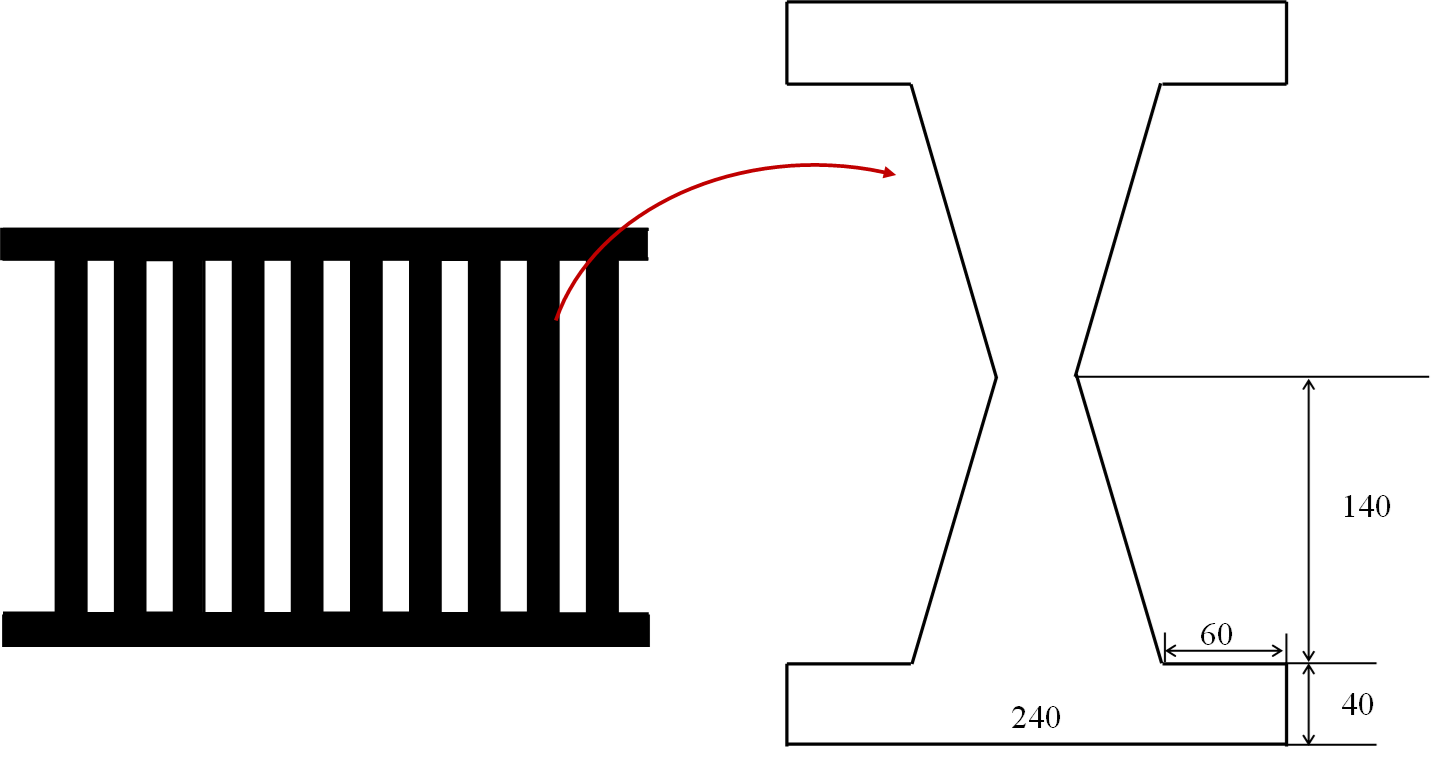
\includegraphics[scale=0.5]{figure/DAMPER/ADAS/2.png}
    \caption{ADAS阻尼器示意图}\label{ADAS2}
\end{figure}
\section{TADAS阻尼器}
ADAS阻尼器的适用性有限,一旦发生横向变形,板将受到张力的影响,导致ADAS的“颈部”X部分容易失效,降低该设备的有效性。
为了改善ADAS阻尼器的缺点,三角板(TADAS)阻尼器被开发出来,TADAS阻尼器通过刚性焊接到顶板,下端简单连接到一个开槽底板,相较于传统的ADAS阻尼器具有不受重力荷载的影响,但构造比ADAS阻尼器复杂。
图(\ref{TADAS1})为一个带有TADAS阻尼器的实验装置\cite{mohammadi2017,kim2016},为常在道路、住房和城市中心建造的一层框架大比例模型,
该框架高3米,跨度4米,框架柱采用标准的双IPE180型钢材,梁的工字截面由三块$4000\times200\times12mm$的钢板连续焊接而成。支撑体系统一采用双$100\times100\times20mm$角度,柱基座使用销连接。
如图(\ref{TADAS2})所示,TADAS阻尼器中的三角形板的上端设为简支固定,下端施加$P=100000$的力。TADAS阻尼器干拌的材料系数为杨氏模量$E=2\times 10^{11}$、泊松比$\nu=0.3$。
图(\ref{TADAS4})为TADAS阻尼器三角形板的弯矩应力云图,
\begin{figure}[H]
    \centering
    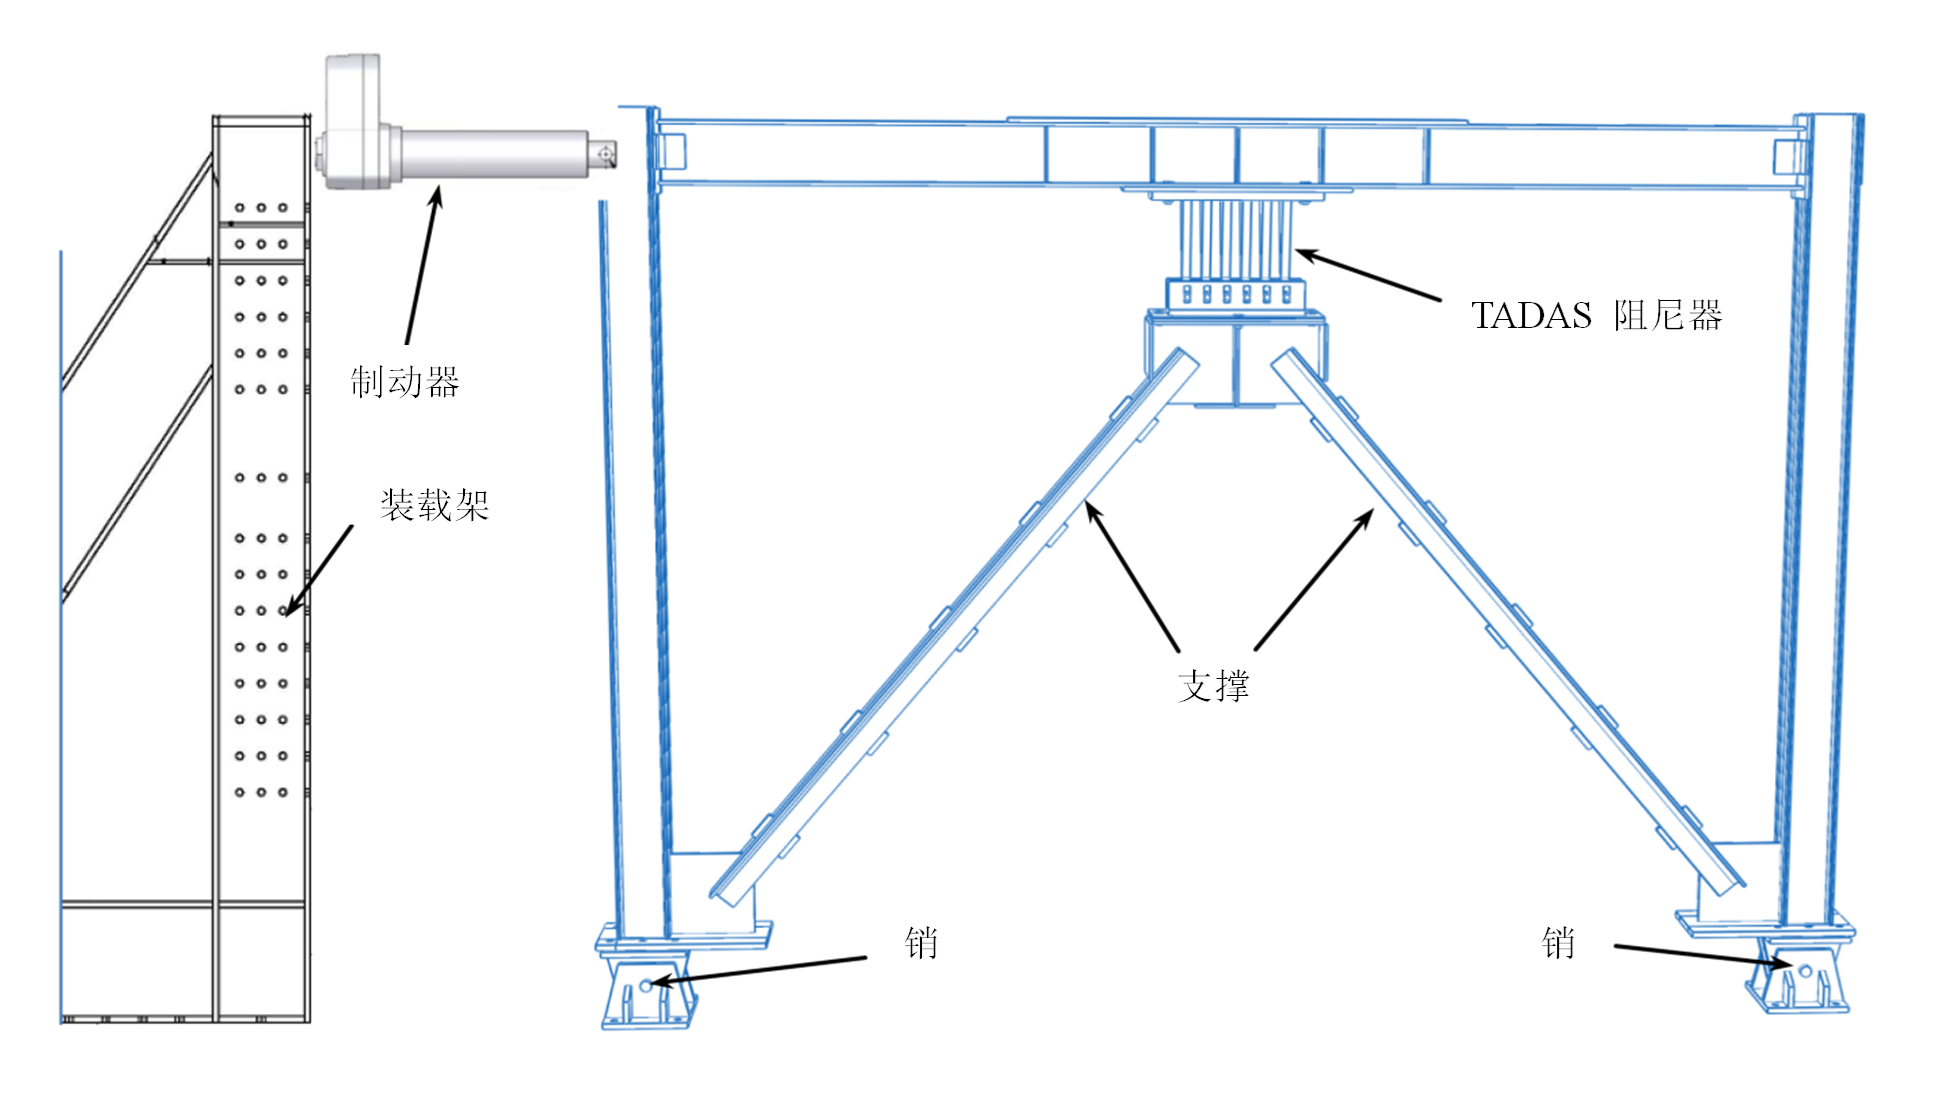
\includegraphics[scale=0.4]{figure/DAMPER/TADAS/1.png}
    \caption{实验装置示意图\cite{mohammadi2017}}\label{TADAS1}
\end{figure}
\begin{figure}[H]
    \centering
    \begin{subcaptiongroup}
            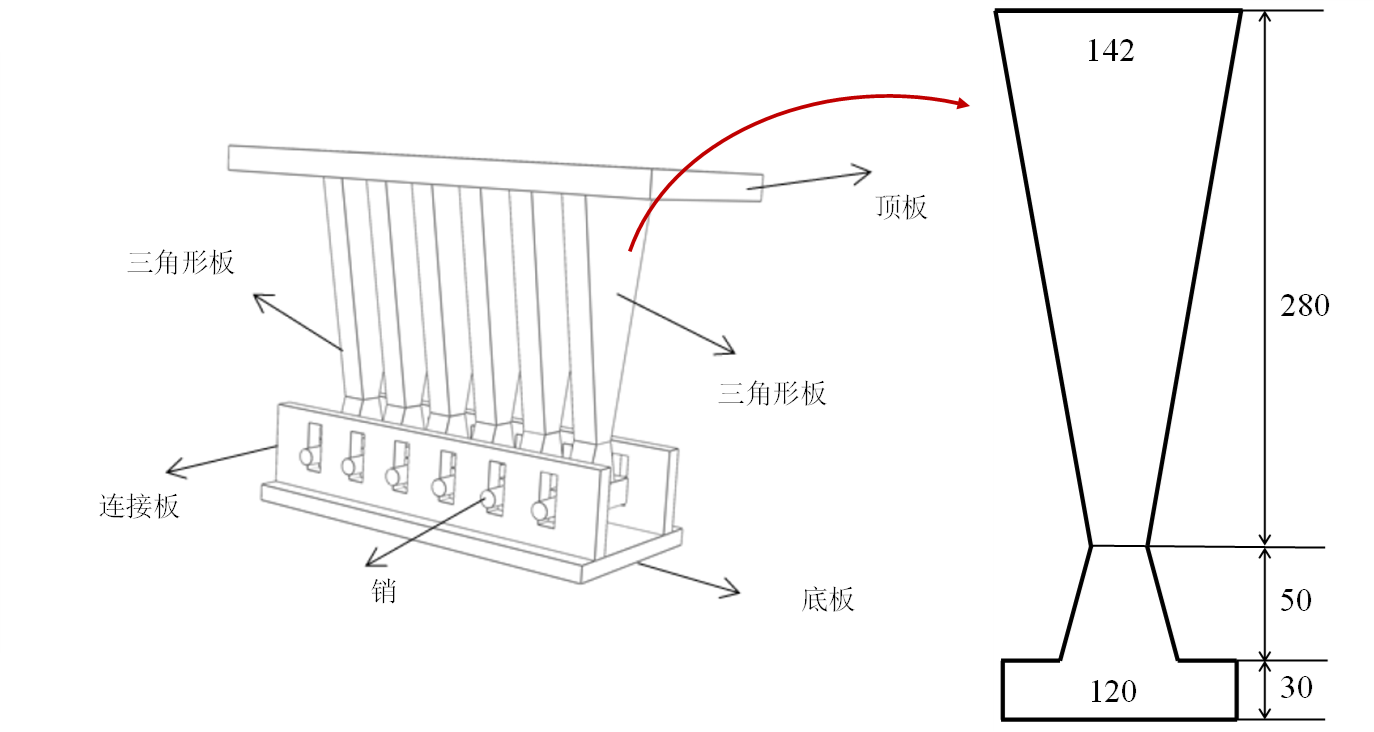
\includegraphics[width=0.69\textwidth]{figure/DAMPER/TADAS/2.png}
            \phantomcaption\label{TADAS2}
            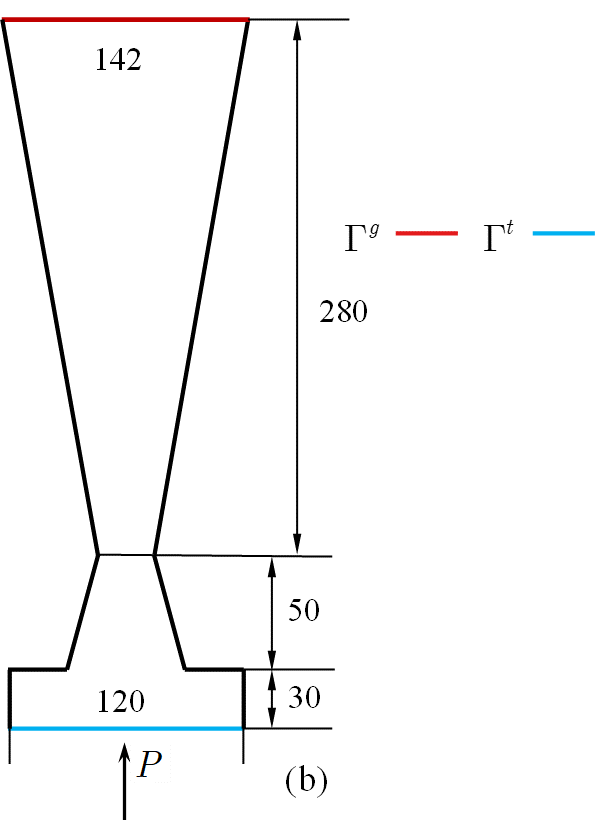
\includegraphics[width=0.29\textwidth]{figure/DAMPER/TADAS/3.png}
            \phantomcaption\label{TADAS3}
            \end{subcaptiongroup}
        \caption{TADAS阻尼器示意图\cite{mohammadi2017}:\subref{TADAS2} 钢板焊接TADAS装置详图;\subref{TADAS3} 三角形钢板横截面图}
    \label{TADAS2}
\end{figure}
\begin{figure}[H]
    \centering
    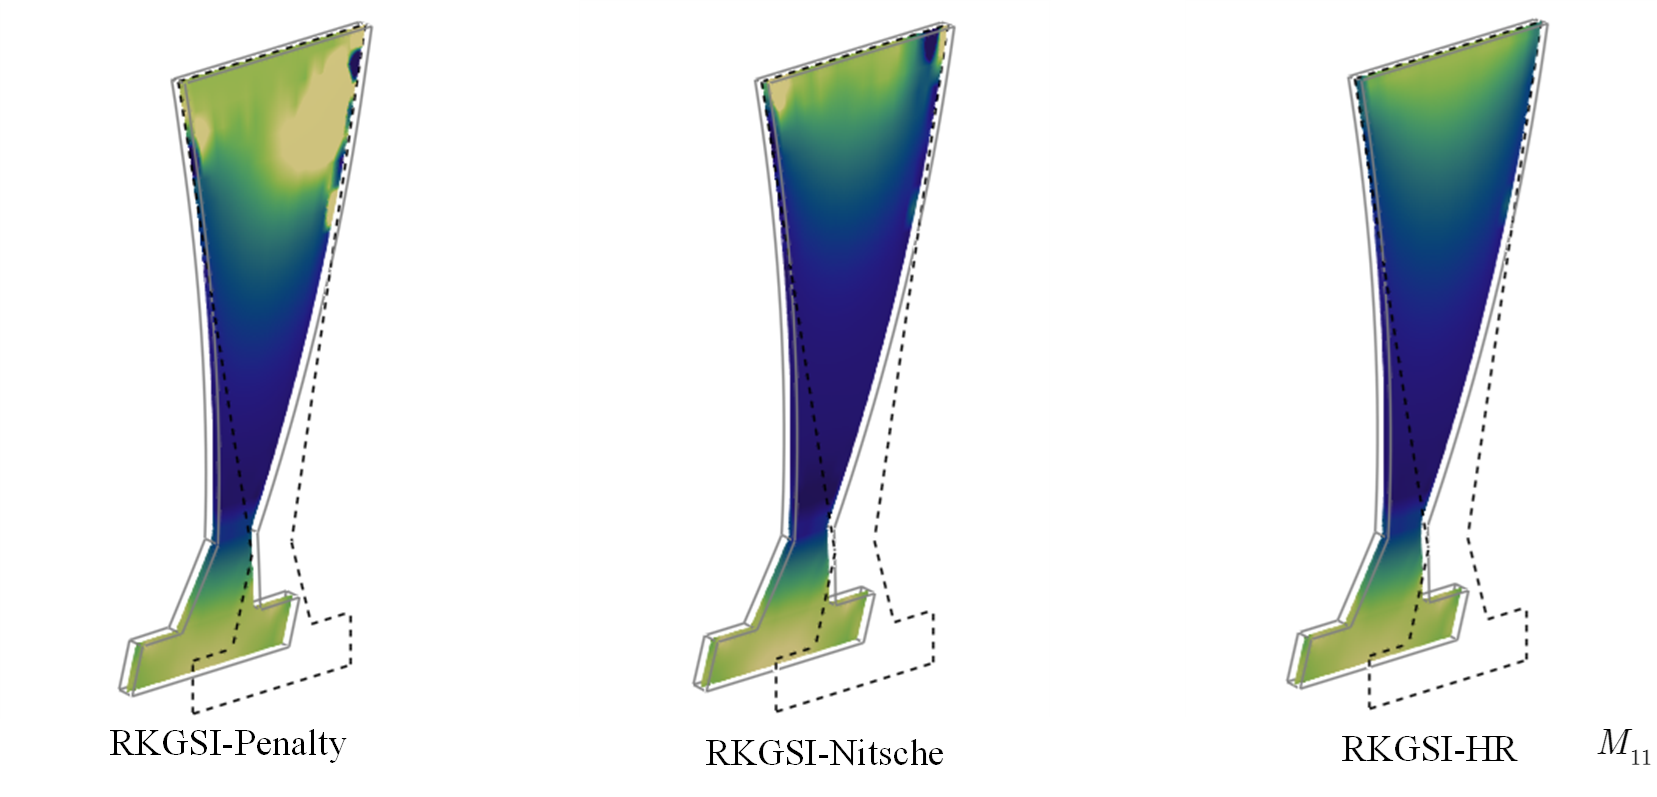
\includegraphics[scale=0.5]{figure/DAMPER/TADAS/M11.png}\\
    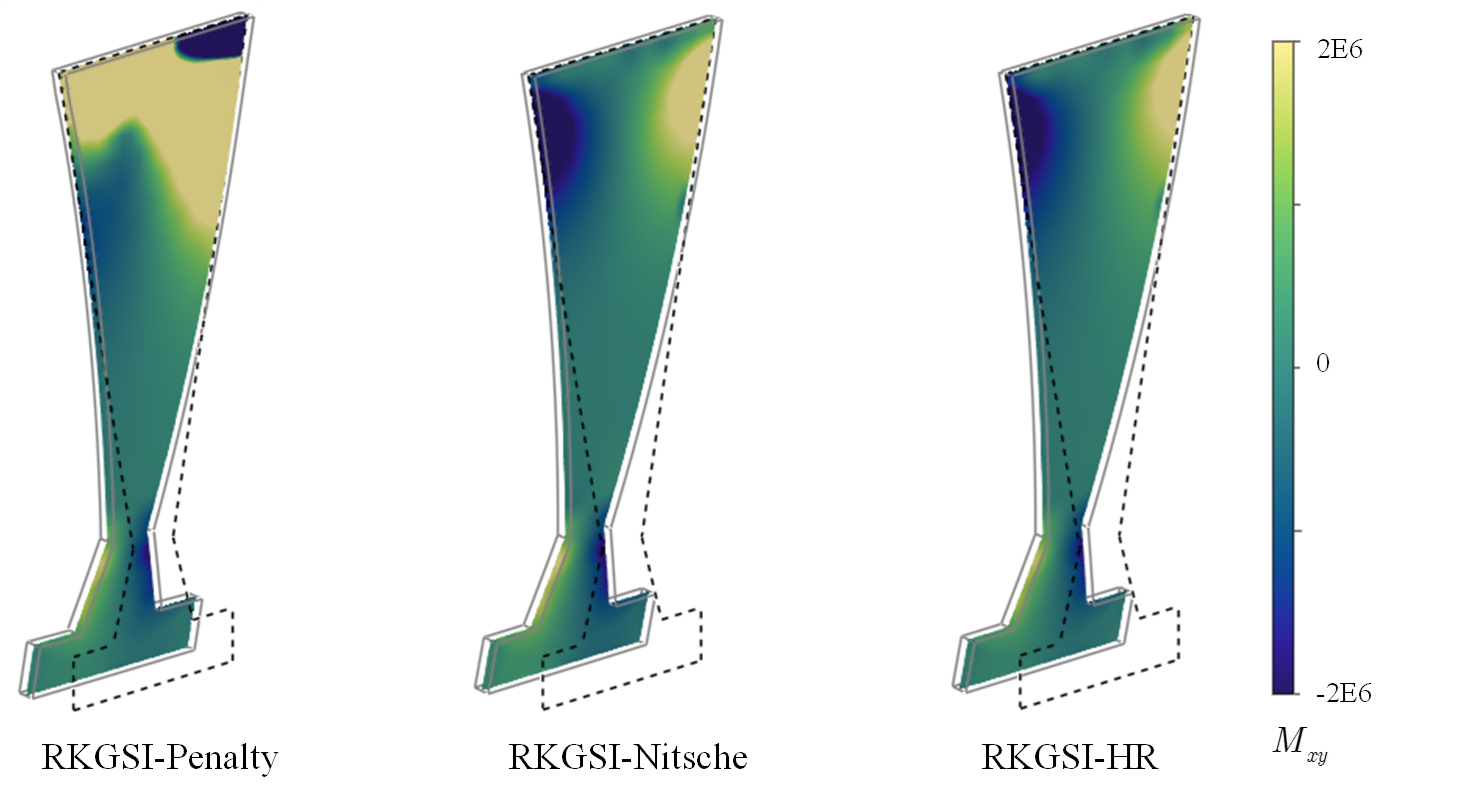
\includegraphics[scale=0.5]{figure/DAMPER/TADAS/M12.png}\\
    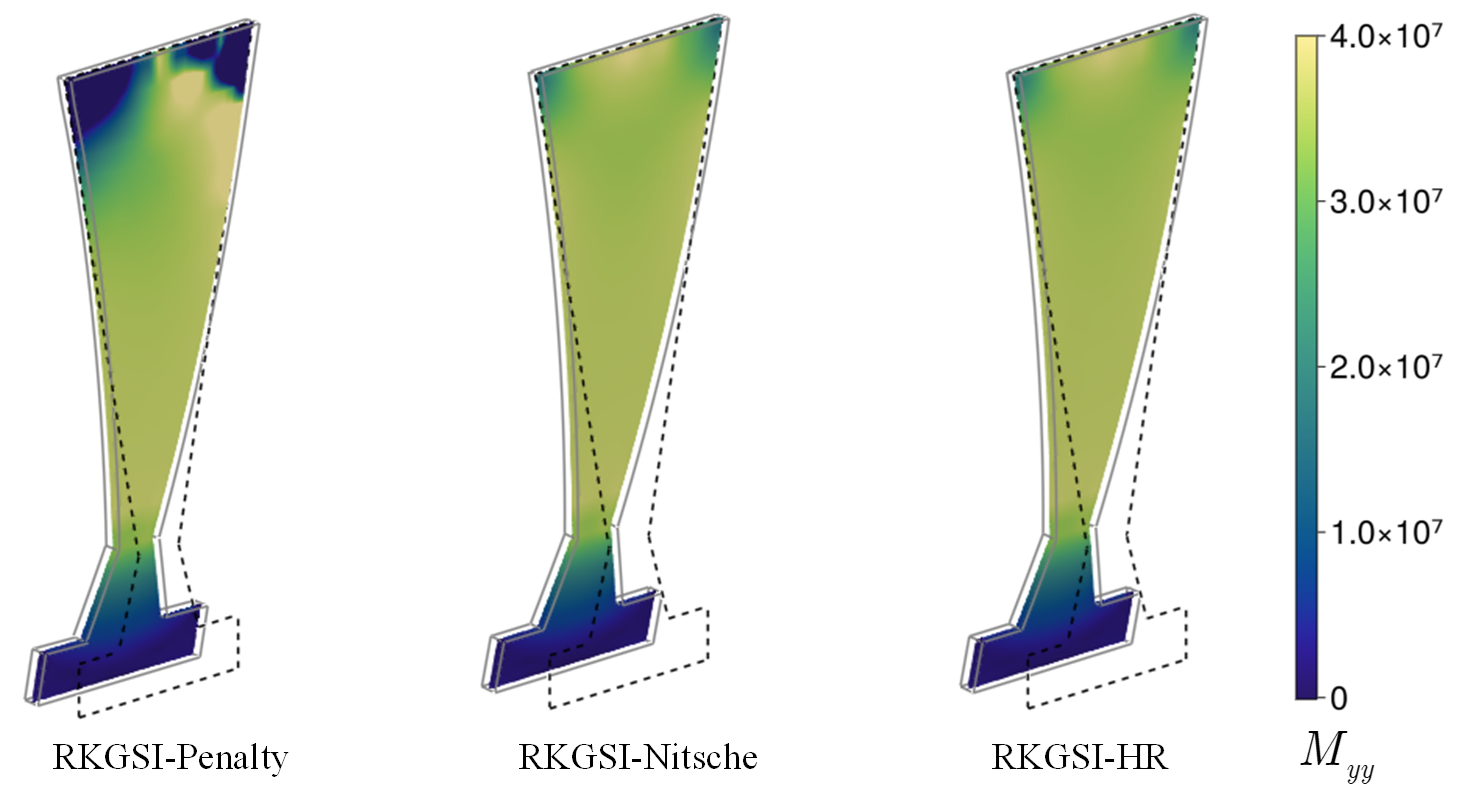
\includegraphics[scale=0.5]{figure/DAMPER/TADAS/M22.png}
    \caption{TADAS阻尼器弯矩云图}\label{TADAS4}
\end{figure}
\section{Slit阻尼器}
狭缝(slit)阻尼器通过在建筑结构中引入缝隙,进而吸收和耗散振动能量,从而有效减少结构的振动响应,同时slit阻尼器的结构相对简单,由一系列平行的缝隙组成,可以根据具体的需求进行设计和调整,并且slit阻尼器通常采用钢材或高性能复合材料制造,具有良好的耐久性和抗腐蚀性能,在工程实践应用中越来越广泛。\par
图(\ref{slit1})为带有slit阻尼器的新型连接体系,梁底部的缝型阻尼器先于主体构件主动塑化,该系统用于震后修复。
如图(\ref{slit2})所示,为了更好的对slit阻尼器进行受力分析,将slit阻尼器的支板理想化,将圆形的末端替换为直线,对silt阻尼器的上端设为简支固定,下端施加$P=100000$的力,该slit阻尼器的材料系数分别为杨氏模量$E=2\times 10^{11}$、泊松比$\nu=0.3$。
图()为slit阻尼器三角形板的弯矩应力云图,
\begin{figure}[H]
    \centering
    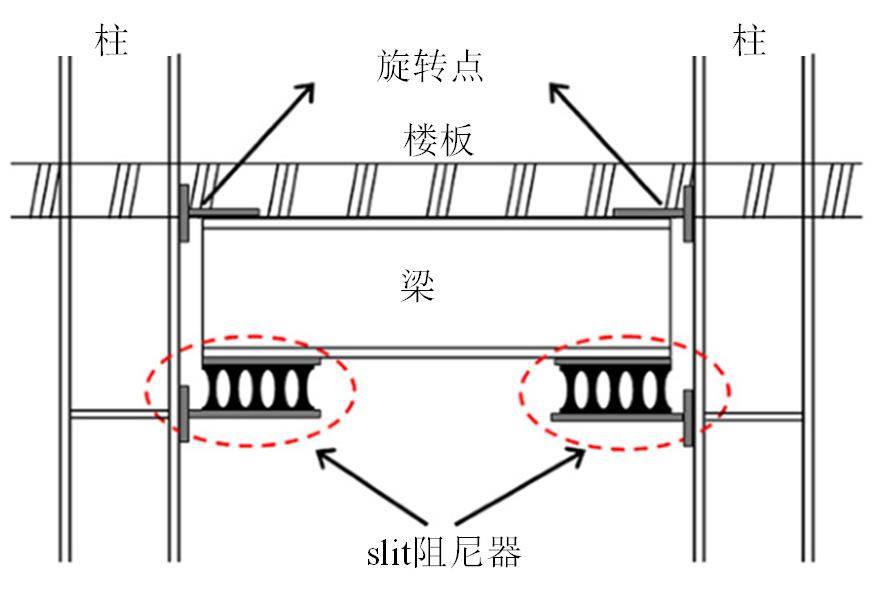
\includegraphics[scale=0.6]{figure/DAMPER/SLIT/1.png}
    \caption{实验装置示意图\cite{oh2009}}\label{slit1}
\end{figure}
\begin{figure}[H]
    \centering
    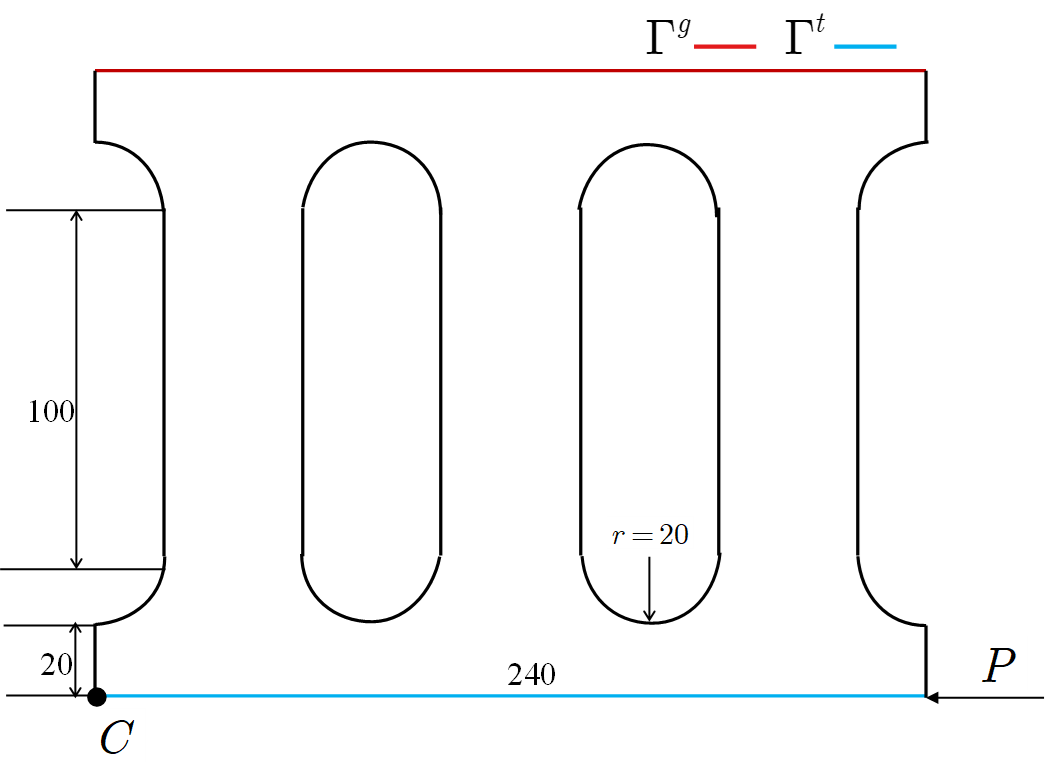
\includegraphics[scale=0.5]{figure/DAMPER/SLIT/2.png}
    \caption{slit阻尼器示意图}\label{slit2}
\end{figure}
\section{小结}
阻尼器在工程应用中起着减震、减振、控制共振等重要应用,因钢、铝合金等金属材料具有高强度和刚性,能够承受较大的负荷并提供稳定的阻尼效果,使得目前阻尼器的原材料多为金属材料。
本章首先分别通过对三种常见的薄板型抗震阻尼器:ADAS阻尼器、TADAS阻尼器和Slit阻尼器进行介绍说明,随后对常见的实验装置中该三种的阻尼器进行建模分析,最后采用不同的本质边界条件施加方法:罚函数法、Nitsche法和本论文提出的HR法得到的弯矩云图进行对比分析,
证明所提方法在处理解决工程应用中薄板型抗震阻尼器的数值模拟分析过程中具有较高的计算精度,为薄板型工程应用提供了一种提高计算精度的数值分析方法。

